\section{Clase 2}

\subsection{El Lagrangeano como punto de partida: Vínculos primarios}
Sabemos que a partir de la segunda ley de Newton, si consideramos una partícula sometida a un campo de fuerza, la trayectoria de viene determinada por



\begin{equation}
  \ddot{\vec{r}}=\frac{1}{m}\vec{F}(\vec{r},\dot{\vec{r}},t)
\end{equation}

\begin{wrapfigure}{l}{0.4\textwidth}
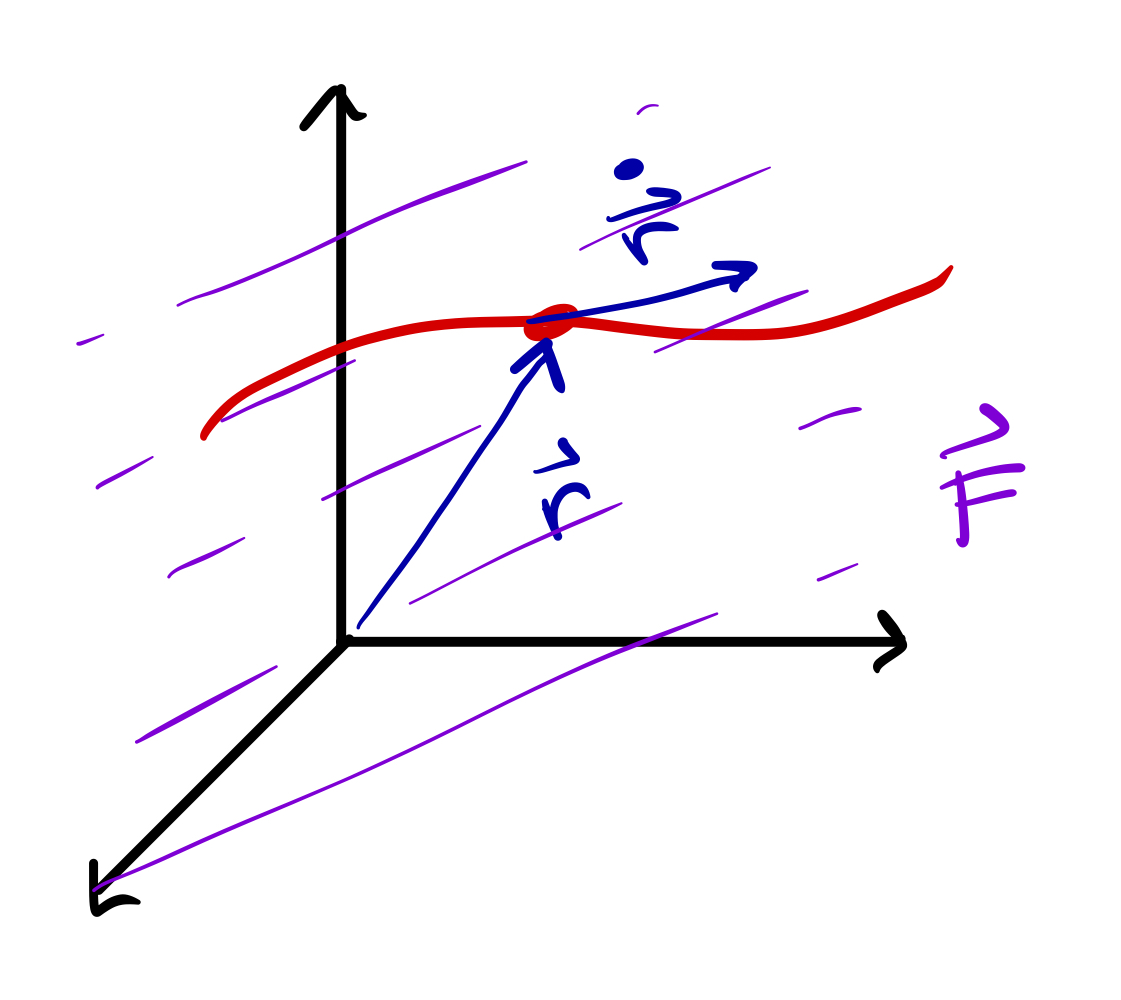
\includegraphics[width=1.0\linewidth]{2-particula} 
\end{wrapfigure}

la cual corresponde a una ecuación diferencial de segundo orden que estará completamente determinada por la fuerza y las condiciones iniciales para la posición $\vec{r}(0)$ y la velocidad $\dot{\vec{r}}(0)$. Luego, el sistema es \textit{determinista}, dado que solo con las condiciones iniciales, podemos determinar el estado del sistema en todo tiempo.


Ahora, si consideramos la descripción de la dinámica a partir de la mecánica analítica, las ecuaciones de movimiento estarán dadas por las ecuaciónes de Euler-Lagrange,
\begin{equation}
  \dv{t}\left(\pdv{L}{\dot{q}^{i}}\right)-\pdv{L}{q^{i}}=0,\qquad L=L(q,\qd,t),\qquad i=1,...,N
\end{equation}
\begin{equation}
  \implies \pdv{L}{q^j}{\qd^{i}}\qd^j+\pdv{\qd^j}\left(\pdv{L}{\qd^{i}}\right)\ddot{q}^j-\pdv{L}{q^{i}}=0
\end{equation}
\begin{equation}
  \implies \left(\pdv{L}{\qd^j}{\qd^{i}}\right)\ddot{q}^j=\pdv{L}{q^{i}}-\pdv{L}{q^j}{\qd^{i}}\qd^j 
\end{equation}
ó
\begin{equation}
 W_{ij}(q,\qd )\ddot{q}^j=\pdv{L}{q^{i}}-\pdv{L}{q^j}{\qd^{i}}\qd^j 
\end{equation}
donde
\begin{equation}
  W_{ij}=\pdv{L}{\qd^j}{\qd^{i}}
\end{equation}
es conocida como la \textit{matriz Hessiana}.

Podríamos concluir que cuando exsten simetrías de gauge, entonces $\det (W)=0$. Este tipo de sistemas son conocidos como \textit{sistemas singulares}.

\begin{ej}
	Consideremos el siguiente Lagrangeano:
	\begin{equation}
  L(q,\qd )=\frac{1}{2}\dot{x}^2+\dot{x}y+\frac{1}{2}(x-y)^2
\end{equation}
entonces $N=2$, donde las coordenadas generaliadas y las velocidades generalizadas son
\begin{equation}
  q^{i}=(x,y),\qquad \qd^{i}=(\dot{x},\dot{y})
\end{equation}
La matriz Hessiana viene dada por
\begin{equation}
  W_{ij}=\mqty(\dfrac{\partial^2L}{\partial\dot{x}\partial\dot{x}} &&&\dfrac{\partial^2L}{\partial\dot{x}\partial\dot{y}} \\\\\dfrac{\partial^2L}{\partial\dot{y}\partial\dot{x}} &&&\dfrac{\partial^2L}{\partial\dot{y}\partial\dot{y}} )=\mqty(1&0\\0&0)
\end{equation}
luego, $\det(W)=0$.

Entonces, podemos afirmar que este Lagrangeano posee simetrías locales (dinámica no determinista). Por inspección, consideremos 
\begin{align}
  \d_sx=\epsilon_1(t),\qquad \d_sy=\epsilon_2(t)
\end{align}
Luego, 
\begin{align}
  \d_sL&=\dot{x}\dot{\epsilon}_1+\dot{\epsilon}_1y+\dot{x}\epsilon_2+(x-y)\epsilon_1-(x-y)\epsilon_2 + \underbrace{\textcolor{blue}{\dot{x}\epsilon_1+x\dot{\epsilon}_1-\dot{x}\epsilon_1-x\dot{\epsilon}_1}}_{\textcolor{blue}{=0}}\\
  &=(\dot{x}+y-x)\dot{\epsilon}_1+(\dot{x}+y-x)\epsilon_2-(\dot{x}+y-x)\epsilon_1+\dv{t}(x\epsilon_1)\\
  &=(\dot{x}+y-x)(\dot{\epsilon}_1+\epsilon_2-\epsilon_1)+\dv{t}(x\epsilon_1)
\end{align}
Por lo tanto, la acción es invariante si
\begin{equation}
\boxed{  \epsilon_2=\epsilon_1-\dot{\epsilon}_1}
\end{equation}
Este ejemplo es ilustrativo para mostrar que
\begin{tcolorbox}
	\begin{equation}
		\text{Simetrías internas}\implies\text{Lagrangeano singular}
	\end{equation}
\end{tcolorbox}
\end{ej}

El punto de partida para el formalismo Hamiltoniano es definir los momentos canónicos, dados por
\begin{equation}
  p_i=\pdv{L}{\qd^{i}}
\end{equation}
Consideremos ahora un sistema gobernado por un Lagrangeano de la forma
\begin{equation}
  L=\frac{1}{2}\sum_{i,j=1}^NW_{ij}(q)\qd^{i}\qd^{j}+\sum_i^N\eta_i(q)\qd^{i}-V(q)
\end{equation}
Los momentos canónicos estan dados por
\begin{equation}\label{2.star}
  p_i=\sum_{j}W_{ij}(q)\qd^j+\eta_i(q)
\end{equation}
Consideremos el caso donde $W$ es singular y de rango $R_W$, esta posee $N-R_W$ autovectores asociados al autovalor nulo $\vec{v}_{(\a) }$ con $\a=1,...,N-R_W$.

De \eqref{2.star}, tenemos que
\begin{equation}
  \sum_i v_{(\a) }^{i}W_{ij}(q)=0
\end{equation}
entonces
\begin{equation}
  \sumi \vec{v}_{(\a) }^{i}(q)(p_i-\eta_i(q))=0\qquad (\text{Vínculos $N-R_W$})
\end{equation}
Ahora, llamamos $\{p_a\}$ al conjunto de $R_W$ momenta linalmente independientes, y al conjunto restante $(N-R_W)$ momenta los llamamos $\{p_\a \}$. Entonces la ecuación de los vínculos será
\begin{equation}
  \sum_\b M_\a ^{~\b }(q)p_\b -F_\a (q,\{p_a\})=0
\end{equation}
con
\begin{equation}
  M_\a ^{~\b }(q)=v_{(\a )}^{~\b }(q)
\end{equation}
y
\begin{equation}
  F_\a (q,\{p_a\}) =\sumi v_{(\a )}^{i }\eta_i(q)-\sum_bv_{(\a )}^{b }(q)p_b
\end{equation}
Necesariamente $M$ es una matriz invertible, puesto que de lo contrario habrían más vínculos. 
Puesto que $\det(M)\neq 0$, los vínculos pueden ser escritos en su forma estándar,
\begin{equation}
  \f_\a (p,q)=p_\a -g_\a (q,\{p_a\})=0
\end{equation}
donde
\begin{equation}
  g_\a =\sum_\b (M^{-1})_\a ^{~\b }F_\b (q,\{p_a\})
\end{equation}
Estos son conocidos como \textit{vínculos primarios}, puesto que se obtienen a partir de la definición de las momenta, sin utilizar las ecuaciones de movimiento.

Es el $2N$-espacio de fase, los vínculos definen sub-espacio $\Gamma_p $ de dimensión $2N-(N-R_W)=N+R_W$.

Para poder aplicar el mecanismo de Dirac es fundamental identificar el número exacto de vínculos en la teoría. Esto implica que los vínculos sean funcionalmente independientes y que el número d vínculos sea constante a lo largo del espacio de fase. La región del espacio de fase que satisface estas condiciones es conocida como \textit{sector canónico} de la teoría. Por lo tanto, los sectores canónicos cumplen con:
\begin{enumerate}
	\item condiciones de regularidad, y
	\item condiciones de no degenarción.
\end{enumerate}

%\subsection{Condición de regularidad}
%Si llamamos $z^{i}\equiv (q,p)$ con $i=1,...,2N$ son las coordenadas del espacio de fase $\G $, los vínculos $\f^\a =0$, donde $\a=1,...,M$ definen la superficie de vínculos $\G_p$, la cual viene dada por
%\begin{equation}
%  \G_p=\{\bar{z}\in \G \, |\,  \f^\a(\bar{z})=0, \quad \a=1,...,M <2N\}
%\end{equation}




































